% ---------------------------------------------------------------------
% 2.6 El paradigma P300 Speller
% ---------------------------------------------------------------------
\section[EL PARADIGMA P300 SPELLER]{El paradigma P300 Speller}
\label{sec:speller}

\subsection{Deletreador de Farwell y Donchin}

En 1988 Farwell y Donchin publicaron el sistema que hoy se conoce como P300 Speller o deletreador
de Donchin, aunque en su artículo original no se habla todavía de una BCI sino de una prótesis
mental que busca servir como canal de comunicación para personas cuya discapacidad motora les
impide comunicarse \cite{farwell1988}. El sistema presenta en pantalla una matriz de $6\times6$
celdas que contiene las letras del alfabeto, algunos números y comandos simples; durante su
funcionamiento, las filas y columnas de la matriz se intensifican una a la vez en orden aleatorio,
mientras el usuario concentra su atención en la celda que desea seleccionar, por ejemplo contando
mentalmente las veces que esta se ilumina \cite{farwell1988}. De los doce eventos posibles, seis
filas y seis columnas, solamente dos contienen al carácter objetivo, de modo que estas
intensificaciones funcionan como los estímulos raros del paradigma \textit{oddball} y provocan una
P300 que no aparece en las diez restantes, tal como se representa en la Figura~\ref{fig:matriz}.

\begin{figure}[htbp]
\centering
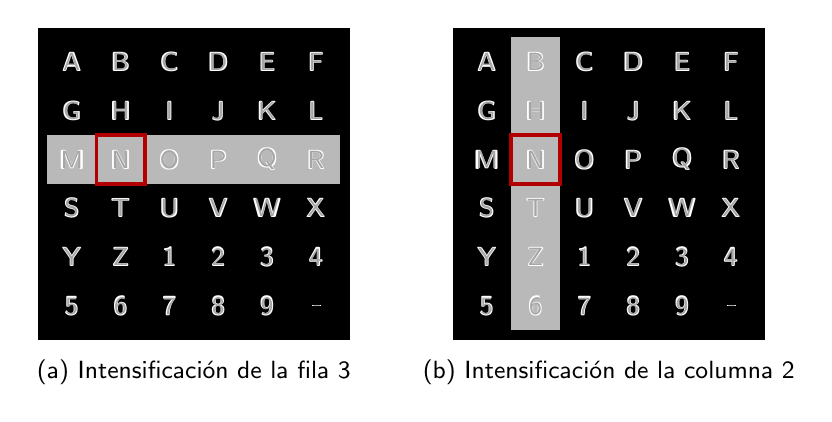
\begin{tikzpicture}[scale=0.62, every node/.style={font=\sffamily\small}]
  \def\letras{{"A","B","C","D","E","F","G","H","I","J","K","L","M","N","O","P","Q","R",
               "S","T","U","V","W","X","Y","Z","1","2","3","4","5","6","7","8","9","\_"}}
  % matriz izquierda: fila 3 intensificada
  \begin{scope}
    \fill[black] (-0.2,-0.2) rectangle (6.2,6.2);
    \fill[gray!55] (0,3) rectangle (6,4);
    \foreach \i in {0,...,35}{
      \pgfmathtruncatemacro{\f}{int(\i/6)}
      \pgfmathtruncatemacro{\c}{mod(\i,6)}
      \pgfmathsetmacro{\l}{\letras[\i]}
      \ifthenelse{\f=2}
        {\node[text=white, font=\sffamily\bfseries] at (\c+0.5,5.5-\f) {\l};}
        {\node[text=gray!70] at (\c+0.5,5.5-\f) {\l};}
    }
    \draw[red!70!black, very thick] (1,3) rectangle (2,4);
    \node[below, align=center] at (3,-0.4) {(a) Intensificación de la fila 3};
  \end{scope}
  % matriz derecha: columna 2 intensificada
  \begin{scope}[xshift=8.5cm]
    \fill[black] (-0.2,-0.2) rectangle (6.2,6.2);
    \fill[gray!55] (1,0) rectangle (2,6);
    \foreach \i in {0,...,35}{
      \pgfmathtruncatemacro{\f}{int(\i/6)}
      \pgfmathtruncatemacro{\c}{mod(\i,6)}
      \pgfmathsetmacro{\l}{\letras[\i]}
      \ifthenelse{\c=1}
        {\node[text=white, font=\sffamily\bfseries] at (\c+0.5,5.5-\f) {\l};}
        {\node[text=gray!70] at (\c+0.5,5.5-\f) {\l};}
    }
    \draw[red!70!black, very thick] (1,3) rectangle (2,4);
    \node[below, align=center] at (3,-0.4) {(b) Intensificación de la columna 2};
  \end{scope}
\end{tikzpicture}
\caption{Matriz de $6\times6$ caracteres del P300 Speller. Si el usuario atiende a la letra N
(recuadro), tanto la intensificación de la fila 3 como la de la columna 2 son eventos objetivo que
provocan una P300; las diez intensificaciones restantes son eventos no objetivo. Elaboración propia
con base en \cite{farwell1988}.}
\label{fig:matriz}
\end{figure}

El sistema original registraba el EEG únicamente en el electrodo Pz y, con cuatro participantes
sanos, alcanzó una exactitud cercana al 95\% con un tiempo promedio de 26 segundos por carácter,
equivalente a 2.3 caracteres o 12 bits por minuto \cite{farwell1988}. Aunque esta velocidad es muy
baja comparada con la escritura convencional, la arquitectura y el principio de operación de este
deletreador siguen siendo la base de la mayoría de los sistemas BCI basados en la P300
\cite{contreras2021}.

\subsection{Parámetros de estimulación}

El desempeño del P300 Speller depende en buena medida de los tiempos con que se presentan los
estímulos. La duración de la intensificación indica el tiempo durante el cual una fila o columna
permanece iluminada; el intervalo entre estímulos (ISI) corresponde al tiempo en que la matriz
permanece sin intensificar antes del siguiente evento; y la suma de ambos define el intervalo entre
inicios de estímulos (SOA). A una secuencia completa de las doce intensificaciones se le llama
repetición, y el número de repeticiones que se realizan antes de decidir el carácter determina el
compromiso entre velocidad y exactitud \cite{krusienski2008}. La Figura~\ref{fig:tiempos}
representa estos parámetros con los valores de la base de datos II de la tercera competencia BCI,
utilizada en este trabajo, en la que cada intensificación dura 100~ms seguida de 75~ms sin
estímulo, y cada carácter se deletrea con 15 repeticiones, es decir, con 180 intensificaciones
\cite{blankertz2006}.

\begin{figure}[htbp]
\centering
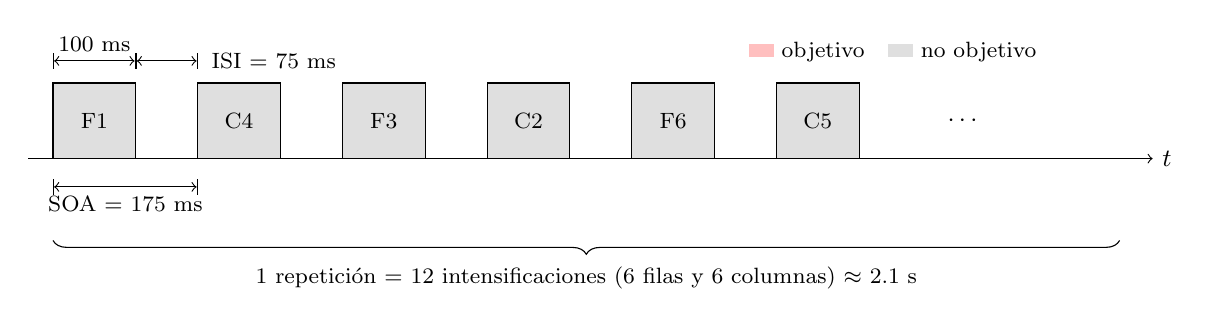
\begin{tikzpicture}[x=1.05cm, y=0.8cm, font=\small]
  % señal de estimulación
  \draw[->] (0,0) -- (13.6,0) node[right] {$t$};
  \foreach \k/\et/\obj in {0/F1/0,1/C4/0,2/F3/1,3/C2/1,4/F6/0,5/C5/0}{
    \pgfmathsetmacro{\xa}{\k*1.75+0.3}
    \pgfmathsetmacro{\xb}{\xa+1.0}
    \ifthenelse{\obj=1}
      {\fill[red!25] (\xa,0) rectangle (\xb,1.2);}
      {\fill[gray!25] (\xa,0) rectangle (\xb,1.2);}
    \draw (\xa,0) rectangle (\xb,1.2);
    \node at ({\xa+0.5},0.6) {\footnotesize \et};
  }
  \node at (11.3,0.6) {$\cdots$};
  % cotas
  \draw[|<->|] (0.3,1.55) -- node[above, font=\footnotesize] {100 ms} (1.3,1.55);
  \draw[|<->|] (1.3,1.55) -- (2.05,1.55); \node[font=\footnotesize, anchor=west] at (2.1,1.55) {ISI = 75 ms};
  \draw[|<->|] (0.3,-0.45) -- node[below, font=\footnotesize] {SOA = 175 ms} (2.05,-0.45);
  \draw[decorate, decoration={brace, amplitude=5pt, mirror}] (0.3,-1.3) -- node[below=6pt, font=\footnotesize, align=center] {1 repetición = 12 intensificaciones (6 filas y 6 columnas) $\approx$ 2.1 s} (13.2,-1.3);
  \node[font=\footnotesize, align=left, anchor=west] at (8.6,1.7) {\tikz\fill[red!25] (0,0) rectangle (0.3,0.2); objetivo\quad \tikz\fill[gray!25] (0,0) rectangle (0.3,0.2); no objetivo};
\end{tikzpicture}
\caption{Parámetros de estimulación del P300 Speller con los valores de la base de datos II de la
competencia BCI III (F = fila, C = columna). Elaboración propia con base en \cite{blankertz2006}.}
\label{fig:tiempos}
\end{figure}

\subsection{Épocas de EEG y decodificación del carácter}

Para clasificar la señal, el registro continuo se divide en segmentos que inician en el instante
de cada intensificación, llamados épocas. Siguiendo la notación de Mercado \cite{mercado2016},
retomada por Contreras \cite{contreras2021}, una sesión de registro puede expresarse como
$x_{i,ch}(n)$, donde $i$ es el número de registro, $ch$ el canal y $n=1,2,\dots,N$ las muestras;
una época se denota como $x^{k,y}_{i,ch}(n)$, donde $k\in\{a,u\}$ indica si se trata de una época
atendida, sincronizada con una fila o columna que contiene al carácter objetivo, o no atendida, y
$y\in\{f,c\}$ indica si la intensificación correspondió a una fila o a una columna.

Una vez que un clasificador asigna a cada época un puntaje $g(\cdot)$ que refleja la probabilidad
de que contenga una P300, el carácter se decide sumando los puntajes de cada fila y cada columna a
lo largo de las $J$ repeticiones y eligiendo aquellas con el valor más alto \cite{rakotomamonjy2008}:
\begin{equation}
\hat{f} = \arg\max_{f\in\{1,\dots,6\}} \sum_{j=1}^{J} g\!\left(x^{f}_{j}\right), \qquad
\hat{c} = \arg\max_{c\in\{1,\dots,6\}} \sum_{j=1}^{J} g\!\left(x^{c}_{j}\right),
\label{eq:decodificacion}
\end{equation}
de modo que el carácter seleccionado es el que se encuentra en la intersección de la fila
$\hat{f}$ y la columna $\hat{c}$. Con esta estrategia, el ganador de la competencia BCI III
alcanzó una exactitud del 96.5\% al utilizar las 15 repeticiones disponibles
\cite{rakotomamonjy2008}.

Cabe destacar que, por la propia estructura del paradigma, el conjunto de épocas está fuertemente
desbalanceado: en cada repetición solo dos de las doce intensificaciones son objetivo, lo que
produce una proporción de una época positiva por cada cinco negativas \cite{cecotti2011}. Si este
desbalance no se considera durante el entrenamiento, un clasificador puede alcanzar una exactitud
aparente cercana al 83\% simplemente prediciendo siempre la clase negativa, razón por la cual las
métricas de evaluación de la Sección~\ref{sec:metricas} deben elegirse con cuidado.

\subsection{Variantes del paradigma}

El paradigma de filas y columnas presenta algunos problemas conocidos. Los errores de adyacencia
ocurren cuando el sistema selecciona un carácter vecino al objetivo, debido a que las
intensificaciones de filas o columnas contiguas también atraen parcialmente la atención del
usuario, y el problema del doble destello aparece cuando la misma fila o columna objetivo se
intensifica dos veces seguidas, de forma que la segunda P300 se atenúa o se traslapa con la
primera \cite{townsend2010}. Para mitigarlos se han propuesto distintas variantes, resumidas en la
Tabla~\ref{tab:variantes}, entre las que destacan el paradigma de tablero de ajedrez de Townsend et
al., que intensifica grupos de caracteres no contiguos \cite{townsend2010}, y el uso de rostros
conocidos superpuestos a los caracteres, con el que Kaufmann et al. obtuvieron ERP de mayor
amplitud y redujeron el número de secuencias necesarias para una selección correcta
\cite{kaufmann2011}.

\begin{table}[htbp]
\centering
\caption{Variantes del paradigma de estimulación del P300 Speller}
\label{tab:variantes}
\small
\begin{tabularx}{\textwidth}{L{3.0cm}YY}
\toprule
\textbf{Variante} & \textbf{Descripción} & \textbf{Ventajas y desventajas} \\
\midrule
Filas y columnas \cite{farwell1988} & Se intensifica una fila o columna completa a la vez. & Solo 12 eventos por repetición; sufre errores de adyacencia y doble destello. \\
Carácter único \cite{guger2009} & Se intensifica un solo carácter a la vez. & P300 de mayor amplitud por ser más infrecuente, pero requiere 36 eventos por repetición y resultó menos exacto en \cite{guger2009}. \\
Tablero de ajedrez \cite{townsend2010} & Se intensifican grupos de caracteres que no comparten fila ni columna. & Reduce errores de adyacencia y doble destello; mayor complejidad en el diseño de los grupos. \\
Estímulos con rostros \cite{kaufmann2011} & Se superpone la imagen de un rostro conocido sobre los caracteres. & ERP de mayor amplitud y menos repeticiones; requiere estímulos visuales más elaborados. \\
\bottomrule
\end{tabularx}
\par\smallskip{\footnotesize Elaboración propia.}
\end{table}

\subsection{Bases de datos públicas}

Gran parte de la investigación sobre detección de la P300 se apoya en bases de datos públicas, lo
que permite comparar métodos bajo las mismas condiciones sin tener que adquirir señales propias.
Las más utilizadas provienen de la segunda y tercera competencias internacionales de BCI, ambas
registradas con 64 canales a 240~Hz con el paradigma de filas y columnas
\cite{blankertz2004,blankertz2006}, mientras que la base de datos de la Escuela Politécnica Federal
de Lausana (EPFL) incluye registros de personas con discapacidad motora con un paradigma de seis
imágenes \cite{hoffmann2008}. La Tabla~\ref{tab:datasets} resume sus características; en el
presente trabajo se emplea la base de datos II de la competencia BCI III, que contiene registros de
dos sujetos con 85 caracteres de entrenamiento y 100 de prueba cada uno.

\begin{table}[htbp]
\centering
\caption{Bases de datos públicas del paradigma P300}
\label{tab:datasets}
\small
\begin{tabularx}{\textwidth}{L{3.3cm}L{1.4cm}L{1.4cm}L{1.4cm}Y}
\toprule
\textbf{Base de datos} & \textbf{Sujetos} & \textbf{Canales} & \textbf{Frec. (Hz)} & \textbf{Paradigma} \\
\midrule
BCI Competition II, conjunto IIb \cite{blankertz2004} & 1 & 64 & 240 & Matriz $6\times6$, filas y columnas, 15 repeticiones. \\
BCI Competition III, conjunto II \cite{blankertz2006} & 2 & 64 & 240 & Matriz $6\times6$, filas y columnas, 15 repeticiones; 85 caracteres de entrenamiento y 100 de prueba por sujeto. \\
EPFL \cite{hoffmann2008} & 8 & 32 & 2048 & Seis imágenes intensificadas de una en una; incluye sujetos con discapacidad motora. \\
\bottomrule
\end{tabularx}
\par\smallskip{\footnotesize Elaboración propia.}
\end{table}
